\chapter{HASIL DAN PEMBAHASAN} \label{bab5}

\section{Proses Identifikasi Kebutuhan Pengguna}
Pengerjaan penelitian ini berorientasi pada kepentingan pengguna dalam memahami makna data direktivitas \bundengan yang telah diukur. Seperti yang sudah dijelaskan sebelumnya, pengguna yang dimaksud adalah orang-orang yang menggeluti kesenian \emph{bundengan}. Secara spesifik, kriteria pengguna untuk sistem visualisasi data direktivitas \bundengan adalah sebagai berikut: \par 

\begin{enumerate}
	\item Menggeluti kesenian musik \emph{bundengan}, baik sebagai pemain ataupun penyelenggara pementasan \emph{bundengan},
	\item Memiliki dan mampu mengoperasikan komputer, dan
	\item Bersedia berkomunikasi secara daring.
\end{enumerate}

Di tengah semakin terancamnya eksistensi \emph{bundengan}, penulis berusaha mencari pengguna yang sesuai dengan kriteria di atas. Pada akhirnya, penulis berhasil berkomunikasi dengan salah satu pemain musik \bundengan di Wonosobo. Pada Gambar \ref{fig:user} diperlihatkan foto calon pengguna bersama \emph{bundengan}. Berikut adalah deskripsi dari calon pengguna sistem visualisasi data direktivitas \emph{bundengan}:

\vspace{0.5 cm}

\begin{tabular}{l l l}
	\textbf{Nama} & : & Muhammad Sa’id Abdulloh \\
	\textbf{Umur} & : & 28 Tahun \\
	\textbf{Domisili} & : & Wonosobo, Jawa Tengah \\
	\textbf{Pekerjaan} & : & Wiraswasta, Pengajar Musik \\
\end{tabular}

\vspace{0.5cm}

Penulis kemudian melakukan wawancara kepada calon pengguna tersebut sebagai bentuk penggalian informasi mengenai kebutuhan pengguna akan sistem visualisasi yang hendak dibangun. Wawancara dilakukan secara daring melalui Google Meet pada Kamis, 2 Desember 2021. Wawancara berlangsung selama kurang lebih satu jam. Wawancara dimulai dengan perkenalan singkat kemudian penulis menjelaskan tujuan utama yang ingin dicapai, yaitu terciptanya pementasan \bundengan yang lebih baik. Dengan memberi pemahaman tersebut harapannya calon pengguna dapat merasakan apa pentingnya keberhasilan sistem ini. Selanjutnya, penulis menjelaskan dari mana asalnya data direktivitas akan disampaikan dalam sistem. Data tersebut dijelaskan sebagai data yang didapat pada penelitian yang dilakukan oleh Kusumaningtyas, Christianto, dan Parikesit sebelumnya \cite{prosidingDirektivitas}. Pada penelitian tersebut telah dihasilkan tampilan yang menunjukkan bagaimana data direktivitas yang terukur (Tabel \ref{tab:prosidingDirektivitas}). Penulis menunjukkan tampilan yang disajikan pada penelitian tersebut kepada calon pengguna untuk mengetahui apakah sajian visual dari data direktivitas \bundengan yang sudah ada telah dapat dimengerti. Hasilnya, calon pengguna sangat kesulitan memahami apa maksud dari tampilan data yang ada pada penelitian sebelumnya. Hal ini membuktikan bahwa perlu adanya perbaikan dalam penyajian data direktivitas \emph{bundengan}. \par 

\begin{figure}[t!]
	\centering
	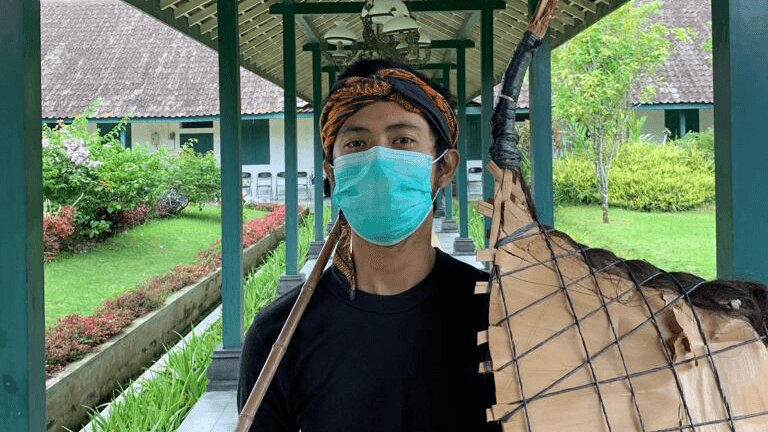
\includegraphics[width=10cm]{Gambar/calon-pengguna.jpg}
	\caption{Calon pengguna.}
	\label{fig:user}
\end{figure}

Setelah mengetahui keluhan calon pengguna mengenai sulitnya memahami data direktivitas bundengan, penulis mulai menggali informasi dari calon pengguna dengan menjelaskan terlebih dahulu maksud dari tampilan visual sebelumnya. Setelah calon pengguna mengerti maknanya, penulis kemudian menanyakan pendapat calon pengguna mengenai keinginannya akan sistem visualisasi data direktivitas bundengan. Pertanyaan yang diajukan berupa bagaimana calon pengguna akan mengoperasikan sistem, apa yang disuka dari sistem yang sudah ada, dan apa yang tidak disuka dari sistem yang sudah ada. Jawaban pengguna atas pertanyaan yang diajukan berupa pernyataan yang kemudian diinterpretasi menjadi kebutuhan yang perlu dipenuhi oleh sistem visualisasi yang dibangun oleh penulis. Pada Tabel \ref{tab:user-needs} diperlihatkan pernyataan yang disampaikan calon pengguna beserta interpretasi maksud pernyataan tersebut sebagai kebutuhan yang perlu dipenuhi oleh sistem. \par 

\begin{table}[b!]
	\centering
	\caption{Interpretasi kebutuhan berdasarkan pernyataan calon pengguna.}
	\begin{tabular}{c p{6cm} p{6cm}}
		\hline
		\textbf{No.} & \multicolumn{1}{c}{\textbf{Pernyataan Calon Pengguna}} & \multicolumn{1}{c}{\textbf{Interpretasi Kebutuhan}} \\
		\hline
		1. & "Saya ingin mengetahui nada mana yang bunyinya merata." & Tampilan nilai TTB dari seluruh frekuensi \\
		\\
		2. & "Saya ingin membandingkan sebaran satu nada dengan nada yang lain." & Pengguna dapat memilih dua atau lebih frekuensi untuk dibandingkan model visualisasinya. \\
		\\
		3. & "Saya merasa nyaman dengan variasi warna yang digunakan" & Rentang nilai TTB perlu diwakili warna dengan perbedaan yang cukup kontras dan bermakna. \\
		\\
		4. & "Saya sulit memahami maksud dari grafik." & Model visualisasi yang digunakan harus mudah dipahami. \\
		\\
		5. & "Saya tidak begitu familiar dengan beberapa istilah dan angka-angka yang ditampilkan." & Perlu adanya petunjuk cara menggunakan sistem. \\
		\hline
	\end{tabular}
	\label{tab:user-needs}
\end{table}


\section{Penentuan dan Perancangan Spesifikasi Sistem Visualisasi}
Berdasarkan hasil identifikasi kebutuhan calon pengguna, diketahui lima kebutuhan yang perlu dipenuhi sistem visualisasi data direktivitas \bundengan ini. Untuk memastikan lima kebutuhan tersebut seluruhnya terpenuhi, perlu adanya rincian metrik/spesifikasi sistem visualisasi yang hendak dibangun. Pada Tabel \ref{tab:specs} diperlihatkan rancangan spesifikasi sistem beserta kebutuhan pada Tabel \ref{tab:user-needs} yang dipenuhi. \par 

\begin{table}[t!]
	\centering
	\caption{Hubungan metrik sistem dengan kebutuhan calon pengguna}
	\begin{tabular}{c p{7cm} c}
		\hline
		\textbf{No.} & \multicolumn{1}{c}{\textbf{Metrik}} & \textbf{No. Kebutuhan} \\
		\hline
		1. & Tampilan data dalam grafik kontur & 1, 3 \\
		\\
		2. & Tampilan data dalam plot pada diagram polar & 1, 4, 5 \\
		\\
		3. & Fitur sorotan untuk beberapa frekuensi alami tertentu & 2 \\
		\\
		4. & Laman bantuan/pengenalan awal program & 5 \\
		\hline
	\end{tabular}
	\label{tab:specs}
\end{table}

Setelah menentukan beberapa spesifikasi yang perlu ada dalam sistem, penulis kemudian memutuskan akan membangun sistem visualisasi ini berupa perangkat lunak/aplikasi komputer \emph{desktop} yang tersedia pada sistem operasi Windows. Aplikasi berbasis \emph{desktop} dipilih karena performanya yang jauh lebih baik dan pengoperasiannya tidak membutuhkan koneksi internet. Aplikasi ini diberi nama "BundenganDVis", yang merupakan penamaan singkat dari \emph{Bundengan Directivity Visualizer}. \par 

\subsection{Rancangan Laman Bantuan}
Laman bantuan atau pengenalan awal disediakan sebagai panduan lengkap dalam menggunakan sistem. Pada berbagai sistem perangkat keras maupun perangkat lunak, hal ini lebih dikenal sebagai "tutorial penggunaan". Kebingungan pengguna terhadap elemen yang ada pada sistem dapat diatasi dengan adanya panduan ini. Oleh sebab itu, panduan ini perlu dirancang dengan pertimbangan latar belakang dan karakteristik pengguna. Hal ini supaya laman bantuan benar-benar membantu pengguna mengatasi ketidakpahaman akan sistem. Dalam kasus penelitian ini, pengguna memiliki latar belakang kesenian, sehingga pengetahuan mengenai istilah-istilah keteknikan sangatlah minim. Oleh sebab itu, penggunaan bahasa yang tepat dan sederhana perlu diterapkan pada penjelasan di menu panduan. Laman bantuan BundenganDVis akan mencakup informasi mengenai \bundengan seperti apa yang diukur, cara menampilkan visualisasi, dan cara memahami makna visualisasi yang ditampilkan. \par 

\subsection{Rancangan Grafik Kontur}
Hasil perekaman data direktivitas \bundengan akan kembali ditampilkan dalam bentuk grafik sebaran warna seperti pada penelitian sebelumnya \cite{prosidingDirektivitas}. Hal ini dilakukan untuk memenuhi kebutuhan pertama dan ketiga. Tampilan data hasil perekaman dalam bentuk peta warna memungkinkan data ditampilkan untuk keseluruhan frekuensi sehingga memudahkan pengamatan kualitas sebaran bunyi untuk berbagai frekuensi. Proses interpretasi yang cepat untuk keseluruhan makna data atau dalam bahasa pengguna "mengetahui nada mana yang bunyinya merata" dapat dicapai dengan tampilan data berbentuk grafik sebaran warna. \par 

\begin{figure}[b!]
	\centering
	\subfigure[]{\label{fig:jet}
\includegraphics[width=12cm]{Gambar/jet.jpg}}
	\subfigure[]{\label{fig:viridis}
\includegraphics[width=12cm]{Gambar/viridis.jpg}}
	\caption{(a) Peta warna jet dan (b) peta warna viridis \cite{cmap}.}
	\label{fig:cmap}
\end{figure}

Meskipun grafik sebaran warna kembali digunakan, ada tiga elemen dari peta warna pada penelitian sebelumnya yang diubah sebagai bentuk peningkatan kualitas model visualisasi. Pertama, jenis peta warna yang akan digunakan sebagai indikator rentang nilai TTB adalah peta warna viridis, bukan peta warna jet. Pada Gambar \ref{fig:cmap} diperlihatkan kedua peta warna tersebut. Peta warna jet adalah peta warna bawaan pada beberapa perangkat lunak dalam menampilkan visualisasi grafis dari data yang memiliki rentang nilai tertentu. Meskipun demikian, penggunaan peta warna ini ternyata bermasalah. \par 

\begin{figure}[t!]
	\centering
	\subfigure[]{\label{fig:slumpring-jet}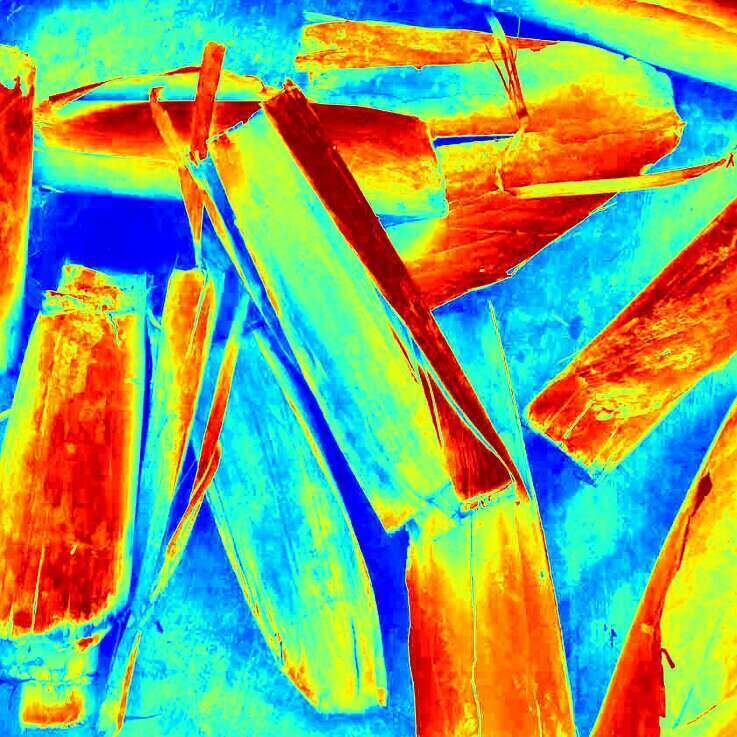
\includegraphics[width=5.5cm]{Gambar/slumpring-jet.jpg}}
	\hspace{1cm}
	\subfigure[]{\label{fig:slumpring-viridis}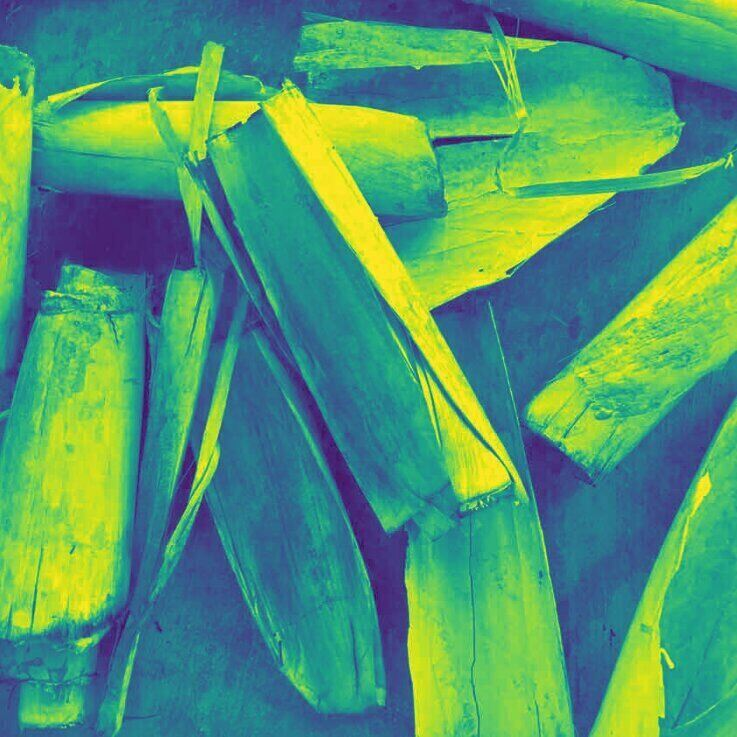
\includegraphics[width=5.5cm]{Gambar/slumpring-viridis.jpg}}
	\caption{Foto \emph{slumpring} dipetakan dengan peta warna (a) jet dan (b) viridis.}
	\label{fig:slumpring-warna}
\end{figure}

Jika sebuah foto dipetakan setiap pixelnya dengan warna yang terdapat pada peta warna jet, foto tersebut tidak lagi dapat diamati sebagai bentuk yang sama dalam penglihatan manusia. Pada Gambar \ref{fig:slumpring-jet} diperlihatkan foto \emph{slumpring} yang sama seperti pada Gambar \ref{fig:slumpring} namun dipetakan dengan peta warna jet. Dapat diamati bahwa bentuk \emph{slumpring} tidak lagi dapat dikenali dengan baik, ditambah jika pengamat tidak pernah melihat foto asli dari \emph{slumpring} tersebut. Berbeda halnya dengan Gambar \ref{fig:slumpring-viridis}, di mana foto \emph{slumpring} yang dipetakan dengan peta warna viridis tetap dapat dikenali bentuknya. Metode evaluasi perseptual dari peta warna ini diperkenalkan oleh Rogowitz dan Kalvin \cite{prosiding-cmap}. Evaluasi dilakukan dengan memetakan beberapa peta warna pada sebuah foto, kemudian meminta pengamat untuk menilai setiap foto. Hasilnya, peta warna tanpa peningkatan kecerahan secara monoton tidak mendapat penilaian yang positif. Tentunya hal ini membuktikan mengapa peta warna jet yang bervariasi pada parameter \emph{hue} tanpa adanya peningkatan luminansi tidak dapat menggambarkan foto dengan baik. Kasus nyata dari hal ini adalah penggunaan peta warna jet pada visualisasi arteri untuk diagnosis penyakit jantung ternyata membutuhkan waktu lebih lama dan secara signifikan lebih banyak terjadi kesalahan \cite{arteri-cmap}. Dengan pertimbangan tersebut penulis memutuskan menggunakan peta warna viridis. Pada Gambar \ref{fig:mesh-bedawarna} diperlihatkan perbedaan grafik sebaran warna yang menggunakan peta warna jet dan viridis. \par 

\begin{figure}[t!]
	\centering
	\subfigure[]{\label{fig:mesh-jet}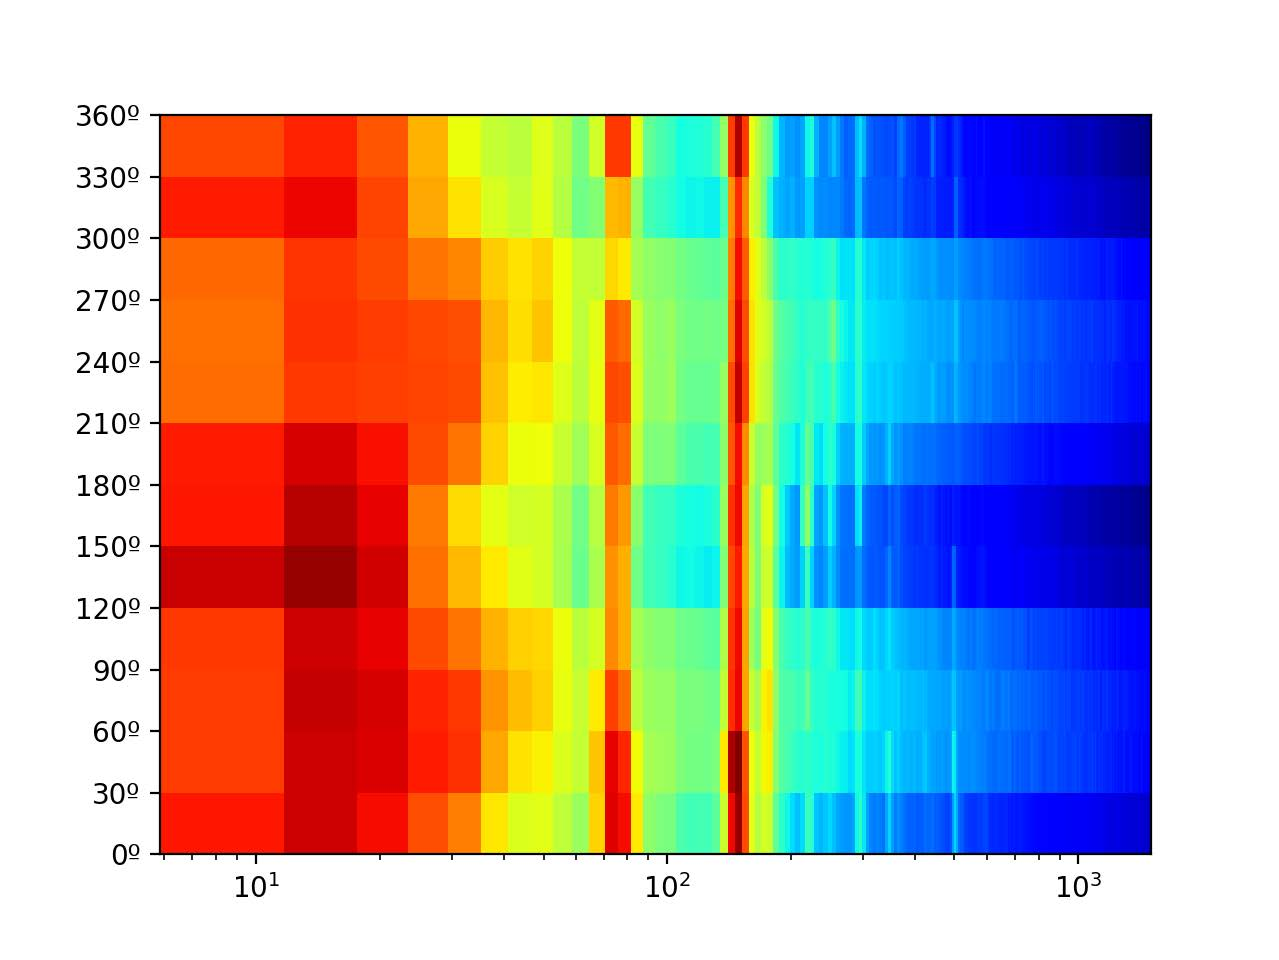
\includegraphics[width=6.5cm]{Gambar/mesh-jet-before.jpg}}
	\subfigure[]{\label{fig:mesh-viridis}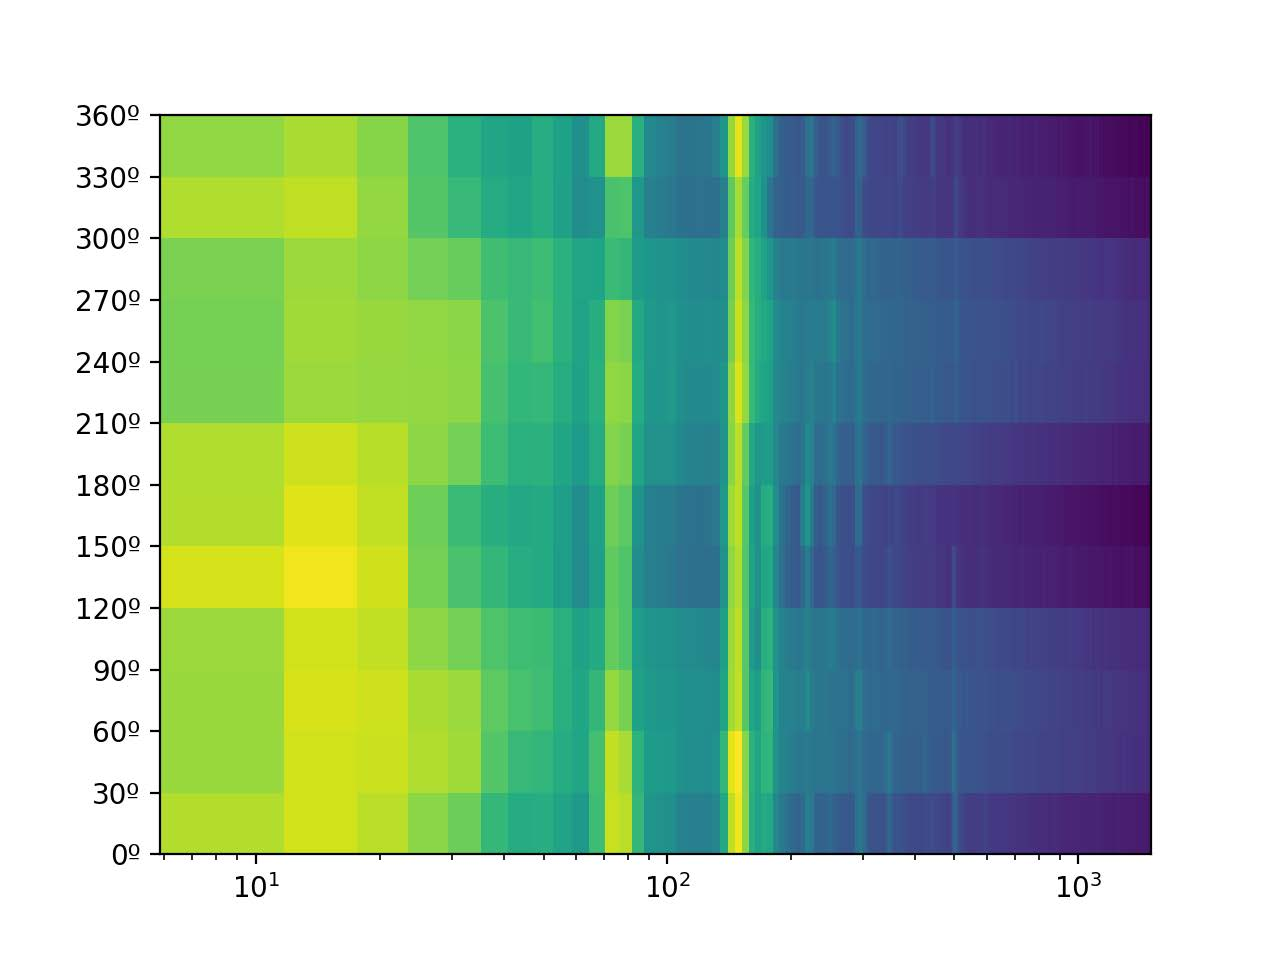
\includegraphics[width=6.5cm]{Gambar/mesh-viridis-after.jpg}}
	\caption{Perbedaan visualisasi data hasil perekaman jika ditampilkan dengan peta warna (a) jet dan (b) viridis.}
	\label{fig:mesh-bedawarna}
\end{figure}

Selain peta warna, elemen dari grafik penelitian sebelumnya yang juga diubah adalah penggambaran tampilan warna untuk setiap koordinat spasial dari frekuensi dan arah data. Pada penelitian sebelumnya grafik sebaran warna terdiri dari kumpulan persegi panjang dengan warna yang berbeda (jaring-jaring warna) sesuai dengan nilai TTB pada frekuensi dan arah tersebut, sedangkan dalam perancangan sistem visualisasi saat ini penulis memutuskan untuk menggunakan tampilan dalam bentuk kontur, yaitu tampilan warna yang memberi kesan tekstur. Sistem visualisasi menampilkan kembali grafik sebaran warna dengan tujuan supaya pengguna dapat mengamati secara utuh bagaimana frekuensi alami \bundengan berada di antara derau sekitar pada saat perekaman. Oleh sebab itu, tampilan dalam bentuk kontur dipilih karena lebih bisa mengekspresikan frekuensi alami \bundengan yang berada di antara derau dengan lebih nyaman dilihat. Perbedaan tampilan jaring-jaring warna dan tampilan kontur diperlihatkan pada Gambar \ref{fig:mesh-kontur}. Pada grafik jaring-jaring warna, nilai TTB untuk setiap pasangan frekuensi dan arah diwakili dengan sebuah persegi panjang dengan warna sesuai nilainya pada rentang peta warna, sedangkan pada grafik kontur satu warna mewakili nilai TTB setiap interval 3 dB sehingga satu warna mewakili lebih dari satu pasangan frekuensi dan arah. \par 

\begin{figure}[t!]
	\centering
	\subfigure[]{\label{fig:mesh-viridis}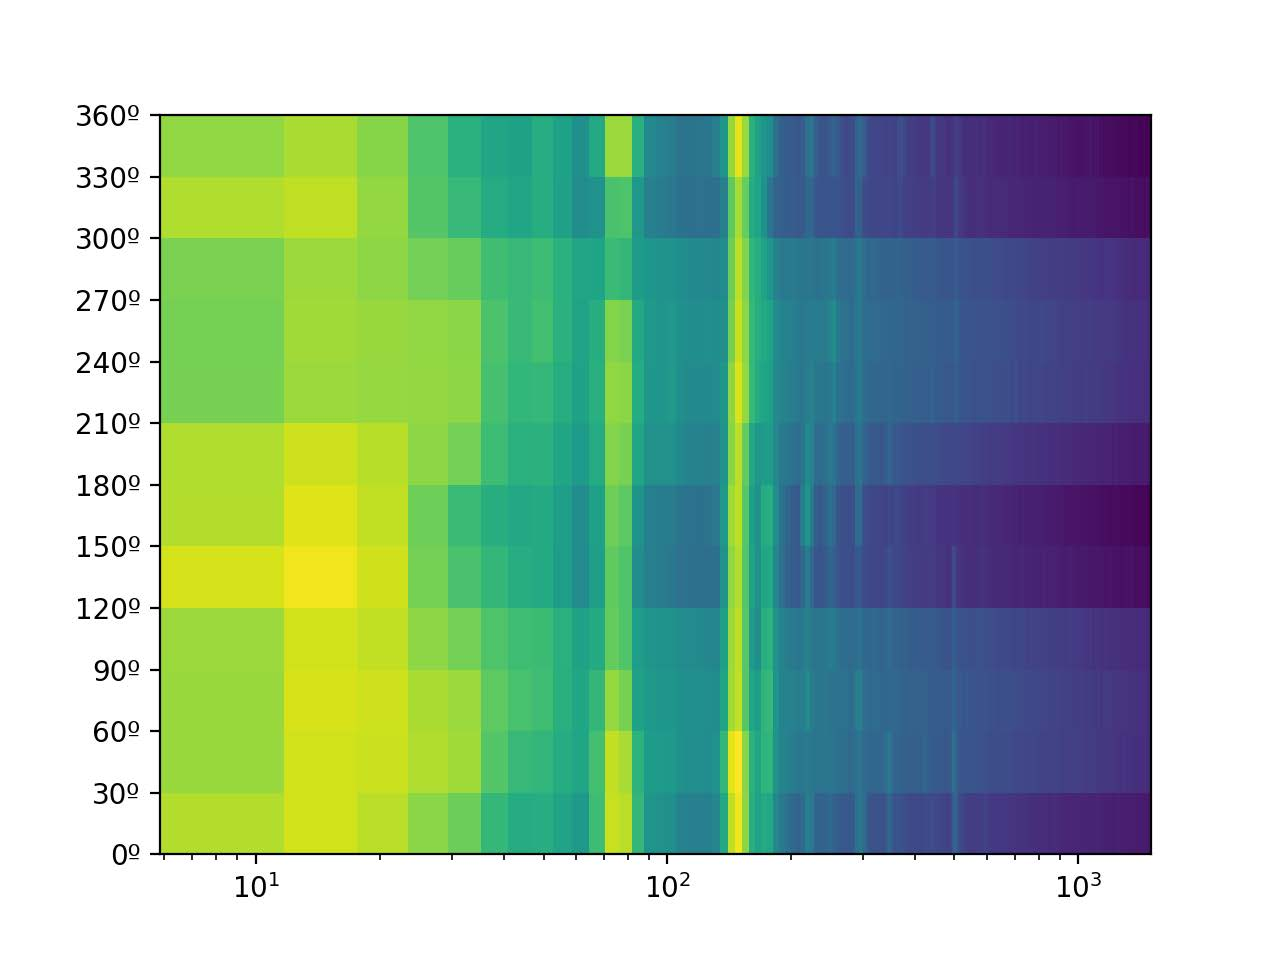
\includegraphics[width=7cm]{Gambar/mesh-viridis-after.jpg}}
	\subfigure[]{\label{fig:kontur-viridis}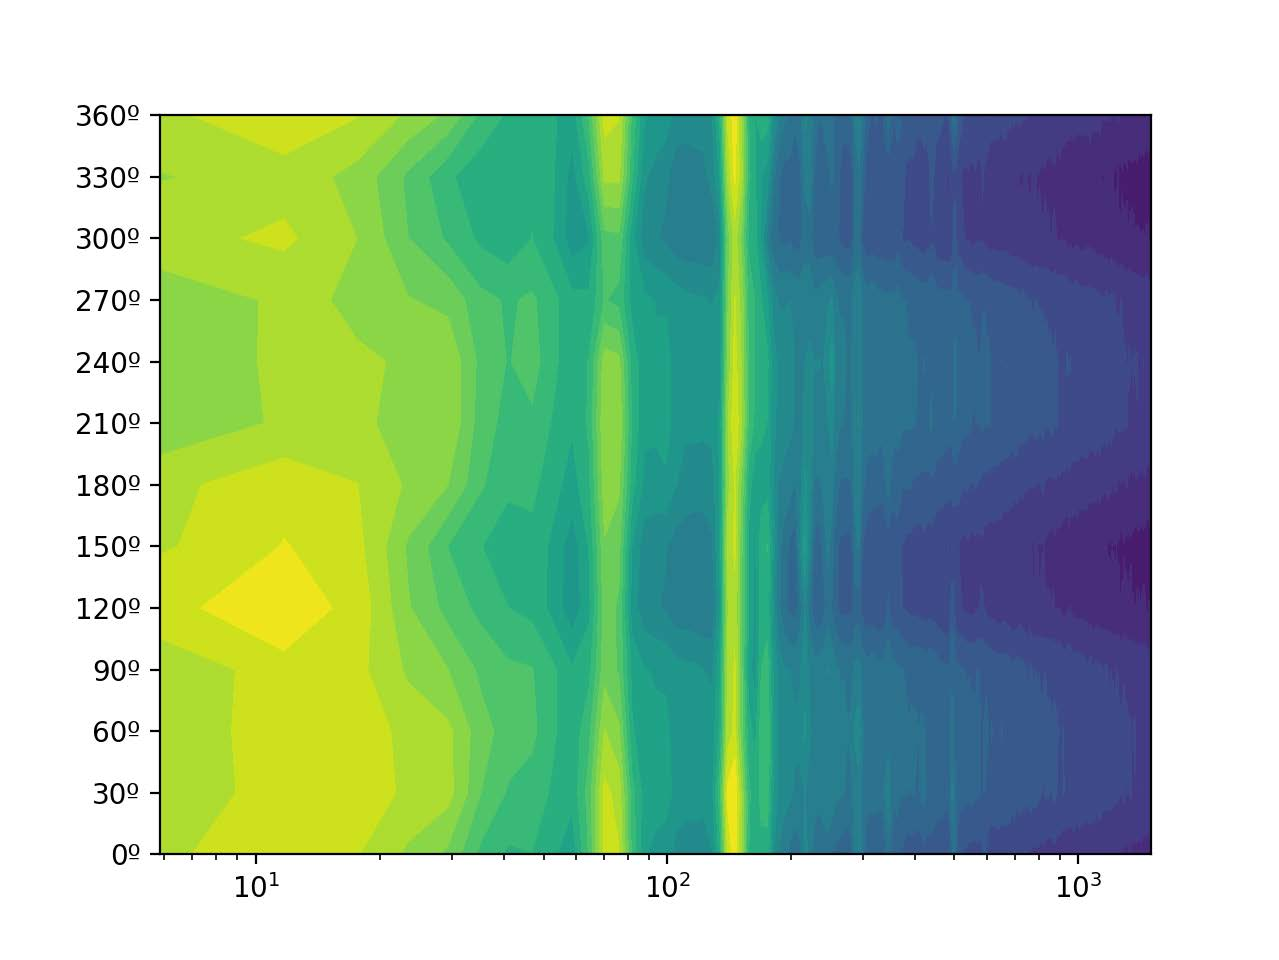
\includegraphics[width=7cm]{Gambar/contour-viridis.jpg}}
	\caption{Perbedaan visualisasi data hasil perekaman jika ditampilkan dengan peta warna viridis dalam bentuk (a) jaring-jaring warna dan (b) kontur warna.}
	\label{fig:mesh-kontur}
\end{figure}

Elemen terakhir yang diubah dari grafik sebaran warna adalah batang warna yang merupakan indikator nilai TTB. Pada penelitian sebelumnya, batang warna berkisar dari warna merah gelap yang mewakili nilai 0 dB sampai dengan biru gelap yang mewakili –60 dB. Batang warna ini menggunakan seluruh warna dari peta warna jet yang diberi indikator setiap –10 dB. Meskipun terdapat indikator untuk rentang yang lebih kecil, pengelihatan manusia tidak mampu membedakan warna dan interpretasi seberapa kerasnya bunyi secara akurat ketika telah dipetakan dalam bentuk grafik. Berdasarkan masalah tersebut, pada batang warna grafik kontur penulis mencacah peta warna viridis menjadi 20 warna yang setiap warna mewakili rentang –3 dB. Pencacahan warna ini bertujuan supaya suatu warna tertentu dapat dengan jelas mewakili rentang nilai TTB. Selain itu, pemilihan rentang –3 dB untuk setiap cacah warna juga bukan tanpa alasan. Jika terdapat dua buah sumber bunyi dengan nilai TTB yang identik (X dB), maka nilai TTB kombinasi kedua sumber bunyi tersebut adalah nilai TTB awal ditambah 3 dB (X+3 dB) \cite{kinsler}. Konsep tersebut digunakan supaya pengguna dapat membayangkan seberapa keras bunyi yang diwakili suatu warna. Jika pengguna memilih satu warna pada grafik, pengguna dapat membayangkan sebuah sumber bunyi, seperti satu senar yang bergetar. Lalu untuk membandingkan seberapa keras bunyi tersebut dengan satu tingkat warna yang lebih terang, pengguna dapat dengan mudah membayangkan dua senar yang bergetar. Jumlah sumber bunyi (dalam hal ini senar yang bergetar) seakan-akan terus berlipat ganda seiring dengan peningkatan warna menuju warna yang lebih terang. Dengan mengubah tiga elemen grafik sebaran warna pada penelitian sebelumnya (peta warna, bentuk penggambaran warna, dan batang warna), didapatkan sebuah grafik kontur warna yang akan ditampilkan dalam BundenganDVis. Pada Gambar \ref{fig:mesh-kontur-bf} diperlihatkan grafik sebaran warna pada penelitian sebelumnya dengan grafik kontur yang dirancang penulis. \par 

\begin{figure}[b!]
	\centering
	\subfigure[]{\label{fig:jet-before}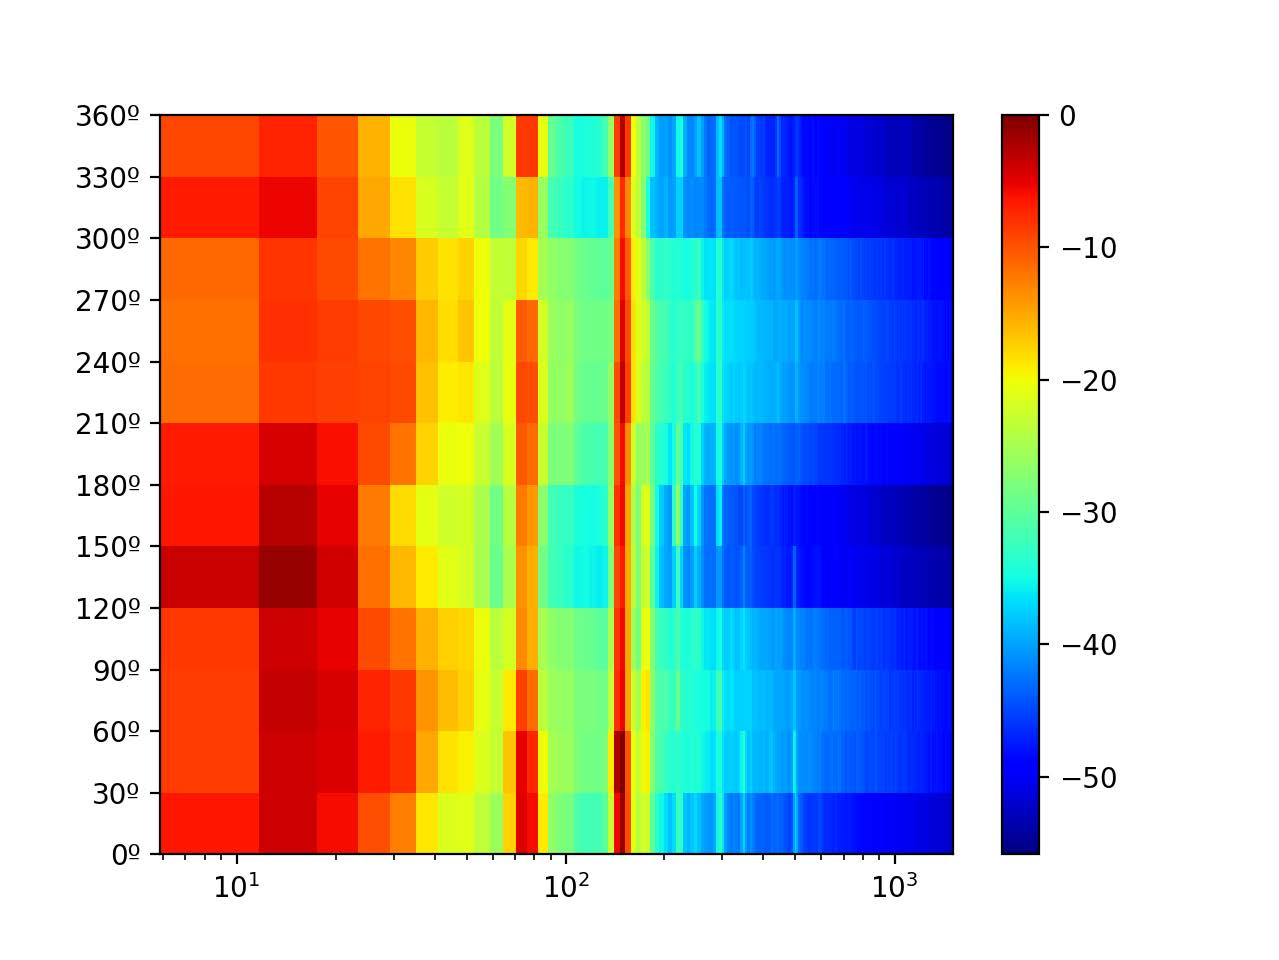
\includegraphics[width=7cm]{Gambar/jet-before.jpg}}
	\subfigure[]{\label{fig:viridis-after}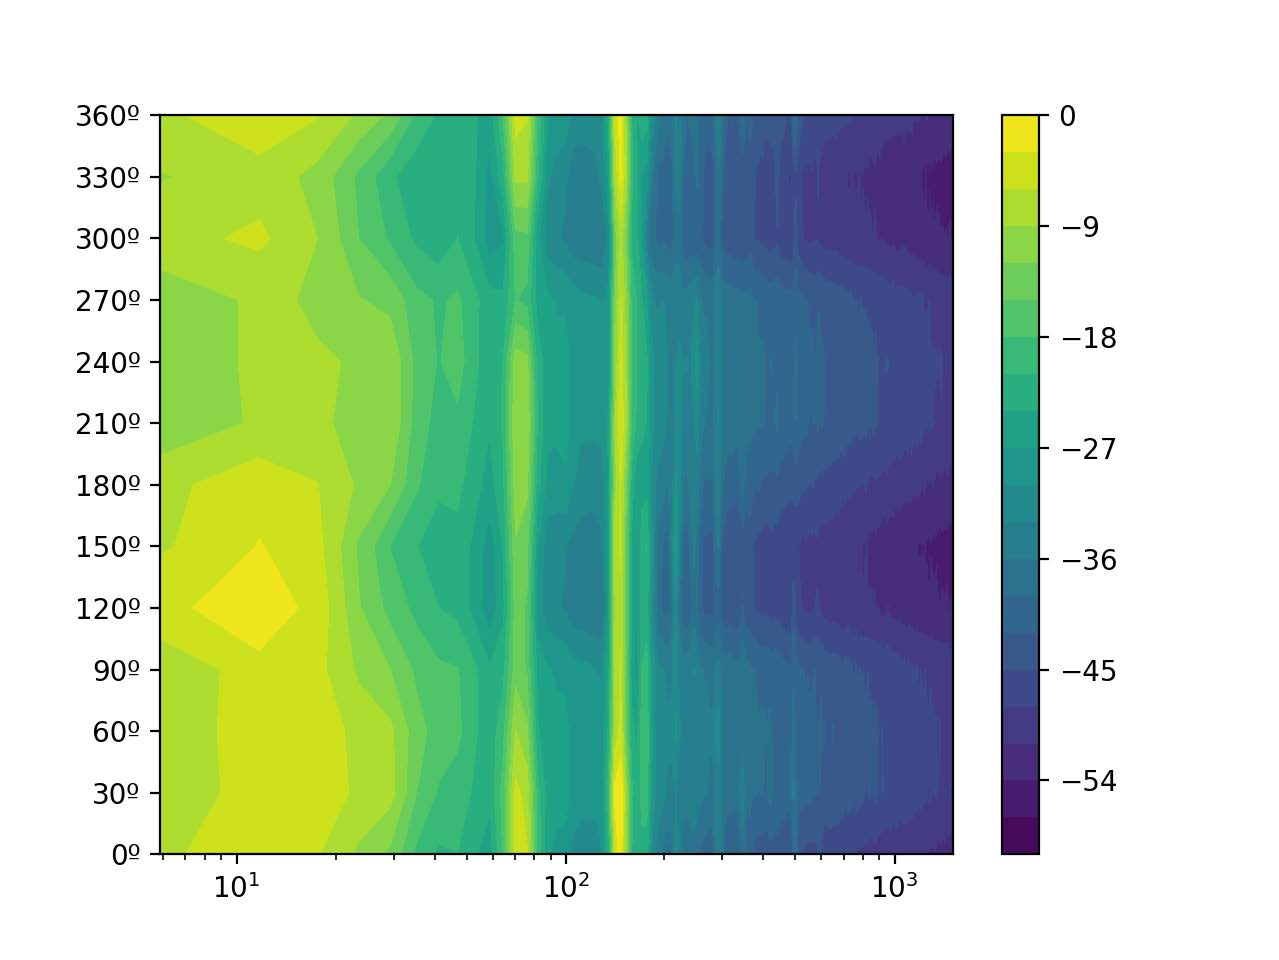
\includegraphics[width=7cm]{Gambar/viridis-after.jpg}}
	\caption{Perbedaan akhir model visualisasi data hasil perekaman pada (a) penelitian sebelumnya [8] dan (b) sistem visualisasi yang hendak dibangun.}
	\label{fig:mesh-kontur-bf}
\end{figure}

\subsection{Rancangan Plot Diagram Polar}
Grafik kontur warna telah dapat menampilkan nilai TTB untuk keseluruhan data yang terekam, tetapi grafik ini kurang optimal jika digunakan untuk mengamati kualitas sebaran bunyi pada frekuensi alami \emph{bundengan}. Oleh sebab itu, perlu adanya model visualisasi lain yang dapat dengan jelas menunjukkan sebaran bunyi pada frekuensi yang spesifik. Jika meninjau kembali berbagai literatur terkait direktivitas, pada umumnya sebuah bunyi pada frekuensi tertentu direktivitasnya digambarkan dalam bentuk plot pada diagram polar. Pemodelan seperti ini telah ditunjukkan pada Gambar \ref{fig:diagramPolarBiola} dan Gambar \ref{fig:contohPolarplotter}. Penggunaan diagram polar juga memungkinkan pengamatan yang lebih spesifik untuk sebaran bunyi pada lebih dari satu frekuensi alami. Oleh sebab itu, selain sebagai sarana pengamatan direktivitas pada frekuensi alami, penggunaan diagram polar juga sekaligus memenuhi kebutuhan perbandingan antar nada/frekuensi alami. \par 


\section{Pembangunan Sistem Visualisasi Data Direktivitas \Bundengan}
Setelah proses perancangan selesai, selanjutnya adalah bagian inti penelitian yaitu pembangunan sistem. Aplikasi BundenganDVis akan terdiri dari dua jenis laman, yaitu laman informasi dan laman fungsional. Laman informasi adalah laman yang menampilkan informasi mengenai BundenganDVis, yaitu laman bantuan, beranda, dan hak cipta. Sedangkan laman fungsional adalah laman yang berisi fungsi sistem yaitu menampilkan data direktivitas \emph{bundengan}, yaitu laman \bundengan 1, \bundengan 2, dan laman untuk membandingkan frekuensi alami kedua \emph{bundengan}. Secara garis besar, proses penggunaan BundenganDVis ditunjukkan pada Gambar \ref{fig:act-diagram}. \par 

Proses pembangunan BundenganDVis terdiri dari penyusunan data direktivitas hasil perekaman, lalu pembuatan algoritma model visualisasi menggunakan data yang telah disusun, terakhir adalah pembuatan GUI BundenganDVis dan pembuatan algoritma kontrol dari aplikasi dengan model visualisasi. \par 

\begin{figure}[h!]
	\centering
	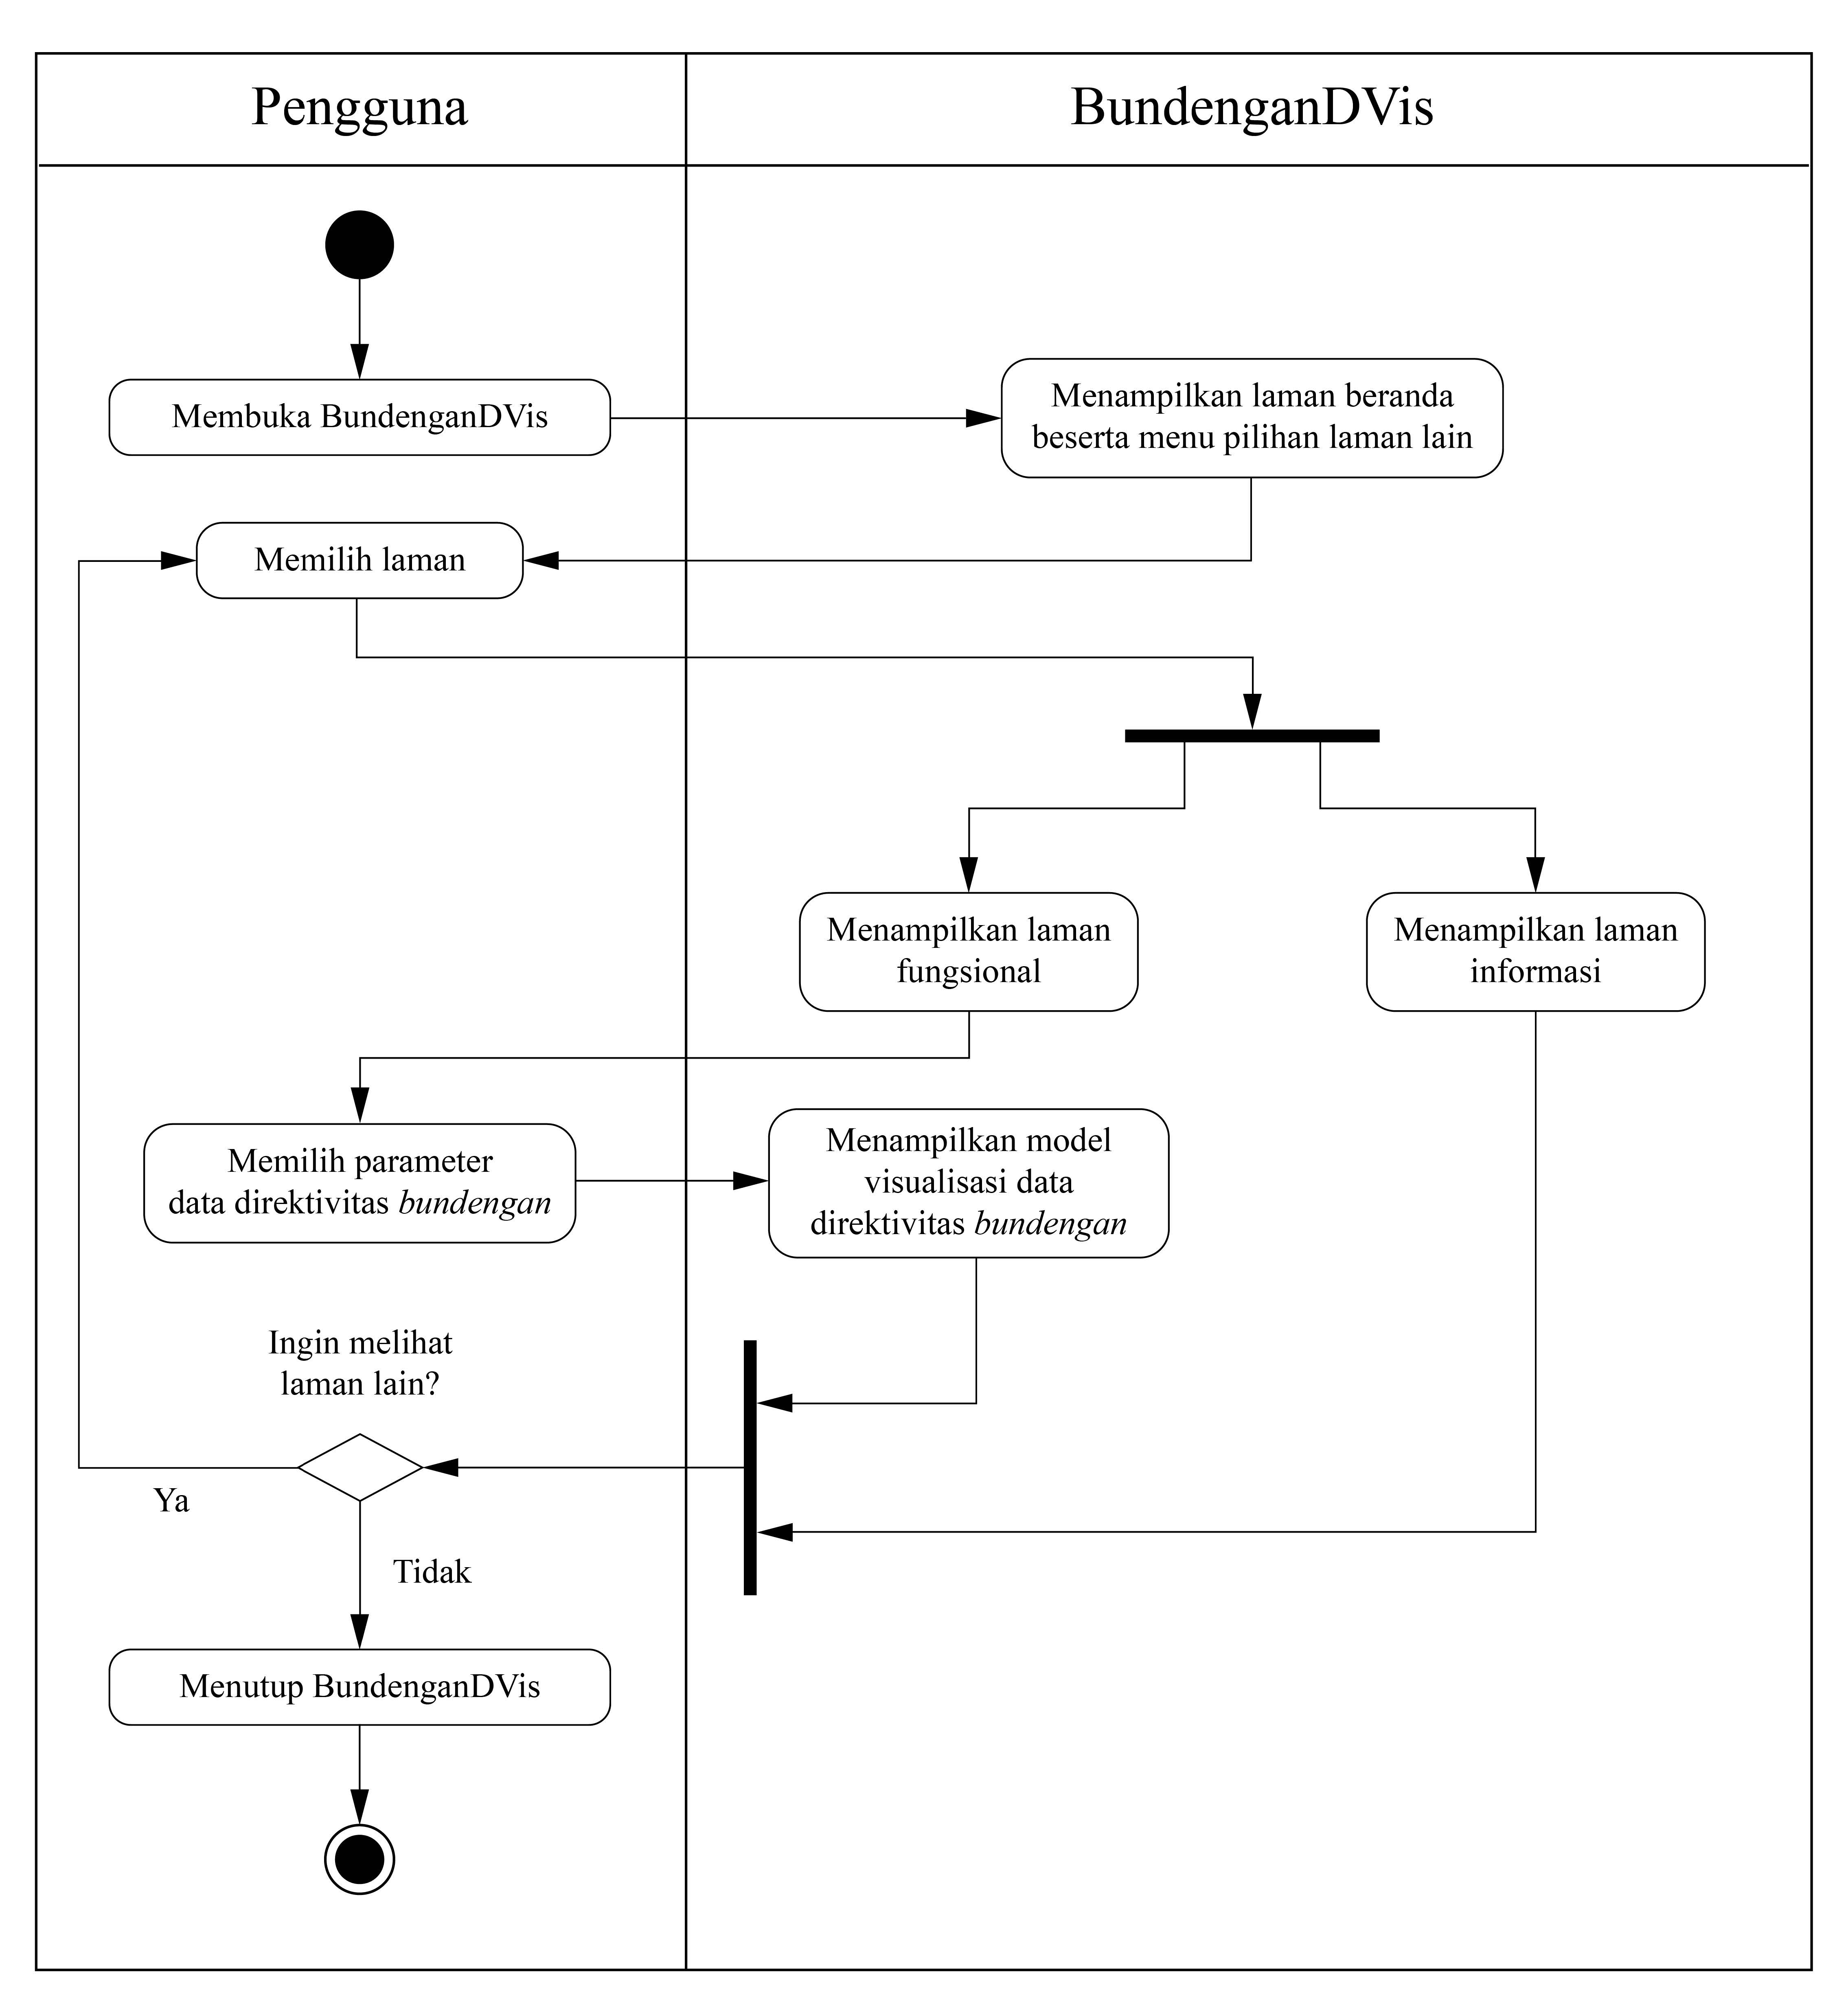
\includegraphics[width= 12.7cm]{Gambar/act-diagram.jpg}
	\caption{BundenganDVis ditampilkan dalam \emph{activity diagram}.}
	\label{fig:act-diagram}
\end{figure}

\subsection{Penyusunan Data}
Data direktivitas \bundengan hasil pengukuran yang dilakukan oleh Kusumaningtyas, Christianto, dan Parikesit diolah menggunakan perangkat lunak Audacity. Dengan perangkat lunak Audacity didapat berkas TTB untuk ukuran \emph{sampling} sebesar 8192. Nilai TTB dan frekuensi pada berkas tersebut adalah nilai yang direpresentasikan oleh grafik sebaran warna pada makalah yang ditulis oleh Kusumaningtyas, Christianto, dan Parikesit. Pembangunan model visualisasi pada BundenganDVis juga akan berdasarkan berkas tersebut. Penulis menerima berkas dengan format ekstensi text (.txt) untuk setiap arah rambat, yaitu 0º (a), 0º (b), 30º, 60º, 90º, 120º, 150º, 180º (a), 180º (b), 210º, 240º, 270º, 300º, dan 330º. Penamaan (a) dan (b) pada berkas arah 0º dan 180º adalah penandaan untuk arah yang terekam dua kali. Seperti yang telah ditunjukkan pada Gambar \ref{fig:bundenganBatasanMasalah}, perekaman hanya dilakukan dengan tujuh mikrofon sehingga untuk mendapatkan data dari seluruh arah maka perlu dilakukan perekaman kedua untuk sisi lain dari \bundengan. Hal ini yang menyebabkan arah 0º dan 180º terekam dua kali. \par 

Pertama-tama penulis merata-ratakan nilai TTB pada berkas 0º (a) dan 180º (b) untuk mendapat nilai TTB pada arah 0º sekaligus 360º, kemudian merata-ratakan nilai TTB pada berkas 180º (a) dan 0º (b) untuk mendapatkan nilai TTB pada arah 180º. Supaya proses pembangunan model visualisasi lebih mudah, data disusun ke dalam dokumen Microsoft Excel. Penulis membuat dua dokumen untuk kedua \emph{bundengan}, masing-masing dokumen terdiri dari empat \emph{sheet} dan 8 \emph{sheet} sesuai dengan jumlah senarnya. Setiap \emph{sheet} senar berisi nilai frekuensi pada kolom pertama dan diikuti dengan nilai TTB untuk arah 0º sampai 360º pada kolom-kolom berikutnya. \par 

Setelah data disusun, dilakukan normalisasi pada nilai TTB. Normalisasi perlu dilakukan karena pada proses perekaman senar tidak dipetik dengan kekuatan yang konsisten sehingga nilai TTB maksimum setiap perekaman berbeda-beda. Hal ini menyebabkan data yang terekam tidak dapat dibandingkan satu sama lain karena basisnya yang tidak sama. Dengan melakukan normalisasi terhadap nilai TTB maksimum pada setiap data, maka nilai TTB maksimum berubah menjadi 0 dB sehingga perbandingan antar data telah dapat dilakukan. Proses ini adalah proses yang juga dilakukan Kusumaningtyas, Christianto, dan Parikesit pada penelitian sebelumnya. \par 


\subsection{Pembuatan Model Visualisasi}
Proses pembuatan model visualisasi dilakukan menggunakan empat pustaka yang tersedia pada bahasa pemrograman Python yaitu Pandas, NumPy, SciPy, dan Matplotlib. Langkah pertama adalah membuat algoritma pemanggilan data direktivitas \emph{bundengan}, yaitu dengan membuat \emph{class} atau objek dengan parameter dua digit angka. Parameter digit pertama mewakili nomor \bundengan sedangkan parameter digit kedua mewakili nomor senar. Pemanggilan objek tersebut akan memberi perintah pembacaan dokumen Microsoft Excel menggunakan pustaka Pandas. Pustaka Pandas memungkinkan akses yang kompleks dan mudah untuk setiap elemen baris dan kolom pada dokumen Microsoft Excel untuk kemudian divisualisasikan. \par 

Seperti yang telah dipaparkan pada bagian perancangan spesifikasi, terdapat dua model visualisasi yang akan dibangun yaitu grafik kontur warna dan plot diagram polar. Sebelum memulai membangun algoritma visualisasi untuk kedua model tersebut, terlebih dahulu dilakukan pemotongan data untuk frekuensi di atas 1500 Hz. Hal ini dilakukan karena nilai TTB untuk frekuensi di atas 1500 Hz sangatlah rendah sehingga perannya dinilai tidak begitu signifikan dalam perancangan pementasan \emph{bundengan}. Untuk membuat model visualisasi grafik kontur, dibuat tiga variabel yang mewakili sumbu $x$, $y$, dan $z$. Nilai frekuensi untuk sumbu $x$ dengan skala logaritmik, nilai arah untuk sumbu $y$, dan nilai TTB untuk sumbu $z$. Untuk model visualisasi plot diagram polar, pertama-tama perlu dilakukan deteksi puncak untuk mengetahui frekuensi alami dari setiap senar \emph{bundengan}. Algoritma deteksi puncak dilakukan menggunakan pustaka SciPy, yaitu pustaka pemrograman Python yang mampu melakukan operasi saintifik seperti pengolahan sinyal. Parameter yang diacu pada proses deteksi puncak ini adalah ketinggian relatif atau dalam pustaka SciPy disebut sebagai \emph{prominence}. Parameter ketinggian relatif sangat cocok digunakan untuk keperluan memisahkan derau dari frekuensi alami \emph{bundengan} karena frekuensi alami berbentuk seperti puncak yang menonjol di antara derau yang berbentuk menyerupai perbukitan, seperti yang ditunjukkan pada Gambar \ref{fig:peak-detect-contoh}. Pada Tabel \ref{tab:hasil-detect} ditunjukkan nilai frekuensi alami yang terdeteksi dari seluruh senar \emph{bundengan}. Nilai TTB dari tiap arah pada frekuensi tersebut kemudian dimuat ke dalam variabel bernama radius, yaitu sumbu $r$ pada diagram polar. \par 

\begin{figure}[h!]
	\centering
	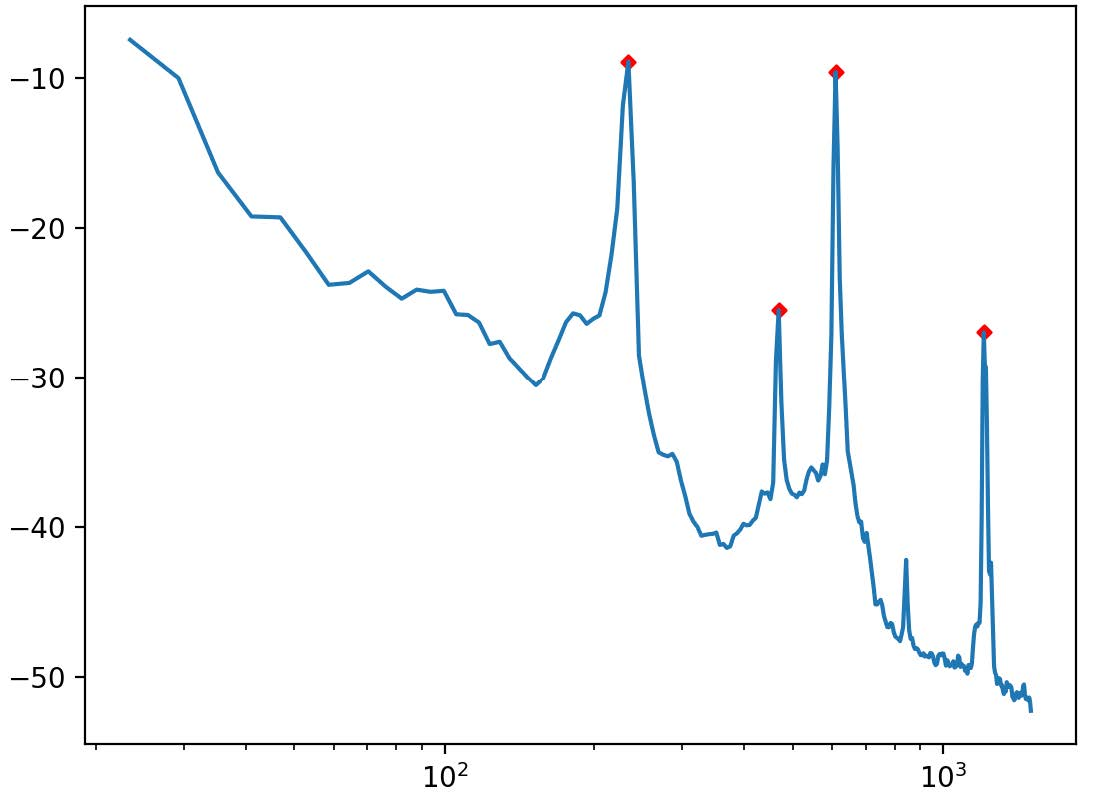
\includegraphics[width=8cm]{Gambar/peak-detect-contoh.jpg}
	\caption{Frekuensi alami yang terdeteksi pada data senar 1 \bundengan 1.}
	\label{fig:peak-detect-contoh}
\end{figure}

\begin{table}[b!]
	\centering
	\caption{Frekuensi alami setiap senar \bundengan berdasarkan deteksi puncak menggunakan pustaka SciPy.}
	\begin{tabular}{l c c c c c}
		\hline
		& & \multicolumn{4}{c}{Frekuensi Alami (Hz)} \\
		& & $f_1$ & $f_2$ & $f_3$ & $f_4$ \\
		\hline
		\multicolumn{6}{c}{Bundengan \#1} \\
		\hline
		Senar 1 && 234,4 & 468,8 & 609,4 & 1207,0 \\
		Senar 2 && 181,6 & 375,0 & -- & -- \\
		Senar 3 && 99,6 & 199,2 & -- & -- \\
		Senar 4 && 70,3 & 146,5 & -- & -- \\
		\hline
		\multicolumn{6}{c}{Bundengan \#2} \\
		\hline
		Senar 1 && 339,8 & 644,5 & -- & -- \\
		Senar 2 && 304,7 & 603,5 & -- & -- \\
		Senar 3 && 287,1 & 603,5 & 1078,1 & 1212,9 \\
		Senar 4 && 228,5 & 451,2 & 1306,6 & -- \\
		Senar 5 && 210,9 & 568,4 & -- & -- \\
		Senar 6 && 169,9 & 334,0 & 527,3 & 1072,3 \\
		Senar 7 && 117,2 & 240,2 & -- & -- \\
		Senar 8 && 99,6 & 205,1 & -- & -- \\
		\hline
	\end{tabular}
	\label{tab:hasil-detect}
\end{table}

Setiap variabel yang dibuat menyimpan nilai dalam bentuk tipe data \emph{array}, yaitu tipe data untuk pustaka NumPy. Penyimpanan dengan tipe data ini bertujuan untuk memudahkan saat memanggil nilai tertentu ketika hendak ditampilkan pada layar visualisasi. Tampilan visualisasi dibuat menggunakan pustaka Matplotlib. Model visualisasi untuk grafik kontur warna telah ditampilkan pada Gambar \ref{fig:mesh-kontur-bf}, sedangkan model visualisasi untuk plot diagram polar ditunjukkan pada Gambar \ref{fig:polar-plot-contoh}. \par 

\begin{figure}[h!]
	\centering
	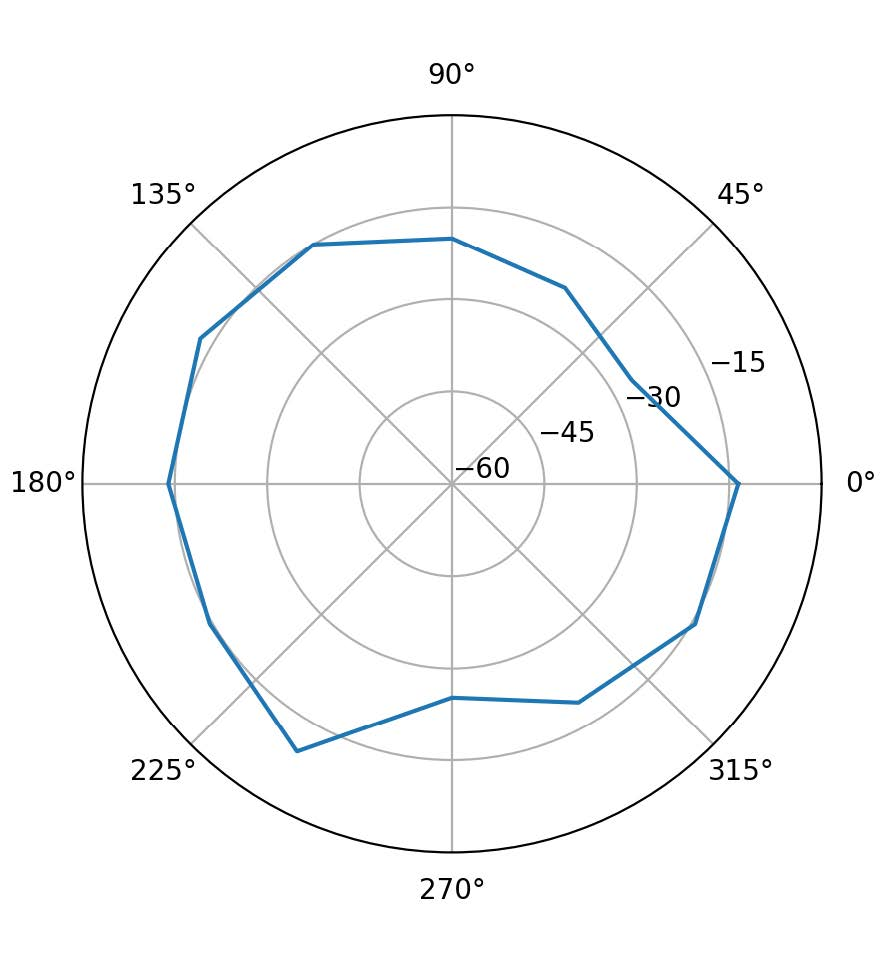
\includegraphics[width=8cm]{Gambar/polar-contoh.jpg}
	\caption{Plot diagram polar frekuensi \overtone pertama senar 1 \bundengan 2.}
	\label{fig:polar-plot-contoh}
\end{figure}

\subsection{Pembuatan GUI Sistem}
Setelah model visualisasi selesai dibangun, selanjutnya dilakukan pembuatan antarmuka sistem yang akan digunakan pengguna dalam pengoperasian BundenganDVis. Secara garis besar antarmuka BundenganDVis terdiri dari menu navigasi pada sebelah kiri dan layar utama di sebelah kanan. Menu navigasi berisi tombol-tombol yang mengontrol tayangan pada layar utama. Berikut ini adalah tombol-tombol pada menu navigasi beserta dengan fungsinya: \par 

\begin{enumerate}
	\item Tombol "Beranda" berfungsi mengarahkan layar utama pada laman beranda.
	\item Tombol "Bundengan \#1" berfungsi mengarahkan layar utama pada laman data mengenai \bundengan 1, yaitu \bundengan yang dimainkan oleh musisi senior.
	\item Tombol "Bundengan \#2" berfungsi mengarahkan layar utama pada laman data mengenai \bundengan 2, yaitu \bundengan yang dimainkan oleh musisi muda.
	\item Tombol "Bandingkan" berfungsi mengarahkan layar utama pada laman fitur perbandingan direktivitas antar frekuensi alami setiap \emph{bundengan}.
	\item Tombol "Bantuan" berfungsi mengarahkan layar utama pada laman bantuan (spesifikasi no. 1).
	\item Tombol "Tentang" berfungsi menampilkan jendela yang berisi informasi mengenai Tim Akustika Musik UGM.
\end{enumerate}

\begin{figure}[h!]
	\centering
	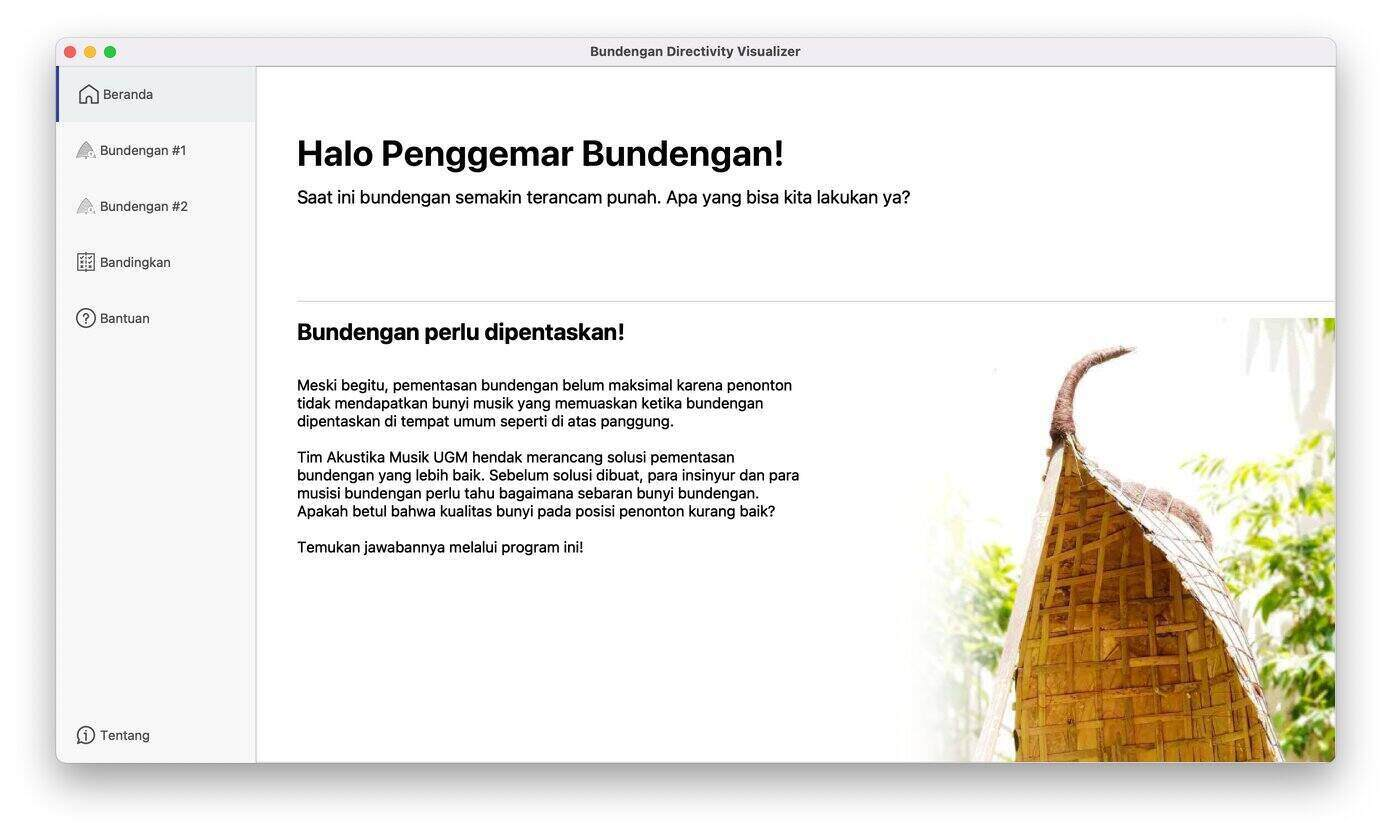
\includegraphics[width=13cm]{Gambar/laman-beranda.jpg}
	\caption{Tampilan laman Beranda BundenganDVis.}
	\label{fig:home-app}
\end{figure}

Laman Beranda adalah laman awal dari BundenganDVis. Layar utama pada BundenganDVis diatur supaya menampilkan laman ini ketika pengguna pertama kali membuka BundenganDVis. Laman beranda berisi penjelasan mengenai tujuan utama dibangunnya program BundenganDVis, yaitu terciptanya pementasan \bundengan dengan kualitas suara yang lebih baik. Penjelasan ini ditampilkan supaya pengguna menyadari bahwa pemahamannya terkait data direktivitas \bundengan sangat diperlukan demi tercapainya konservasi alat musik \emph{bundengan}. Tampilan laman beranda diperlihatkan pada Gambar \ref{fig:home-app}. \par 


Laman Bundengan \#1 dan Bundengan \#2 adalah laman fungsional utama yang menampilkan data direktivitas untuk masing-masing \emph{bundengan}. Setiap laman berisi deskripsi singkat setiap \bundengan beserta foto pada saat dimainkan dan juga tombol untuk mengakses data tiap senar pada \bundengan tersebut. Ketika salah satu tombol senar dipilih, layar utama akan menampilkan tampilan grafik kontur untuk senar tersebut. Selain itu, terdapat pilihan untuk mengganti tayangan pada layar utama menjadi tampilan plot diagram polar untuk melihat bagaimana direktivitas setiap frekuensi alami senar tersebut. Pada Gambar \ref{fig:b2-app} diperlihatkan salah satu laman fungsional utama yaitu laman untuk \bundengan \#2. \par 

\begin{figure}[b!]
	\centering
	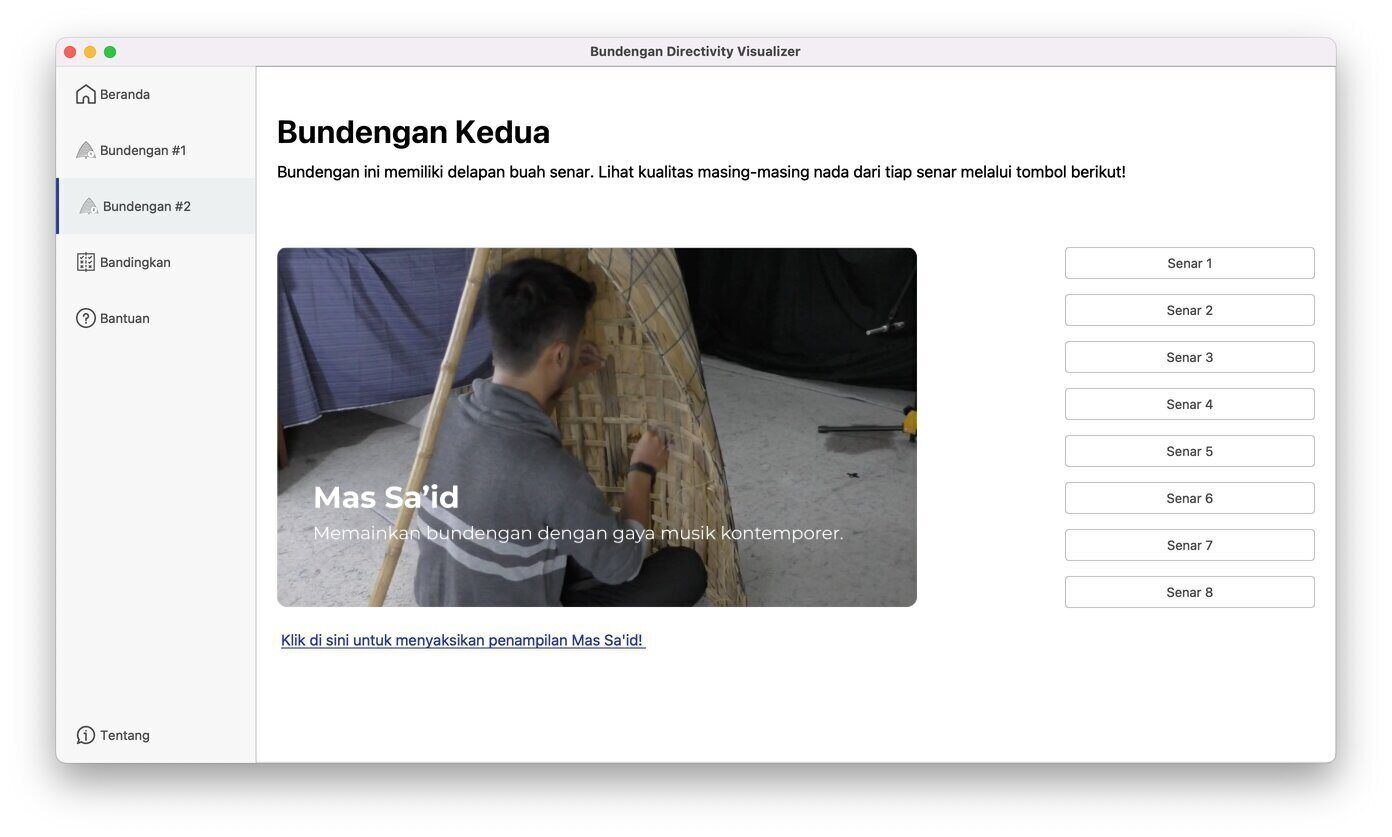
\includegraphics[width=13.5cm]{Gambar/laman-bundengan-2.jpg}
	\caption{Tampilan laman bundengan \#2.}
	\label{fig:b2-app}
\end{figure}

Pada laman Bandingkan, pengguna dapat memilih tiga pilihan perbandingan. Pengguna dapat membandingkan direktivitas dari frekuensi alami antar senar dari \bundengan 1, frekuensi alami antar senar \bundengan 2, atau frekuensi alami antar \emph{bundengan}. Laman ini dibuat karena laman Bundengan \#1 dan Bundengan \#2 tidak dapat digunakan untuk membandingkan frekuensi alami dari dua senar yang berbeda. Laman Bandingkan diperlihatkan pada Gambar \ref{fig:compare-app}. \par 

\begin{figure}[h!]
	\centering
	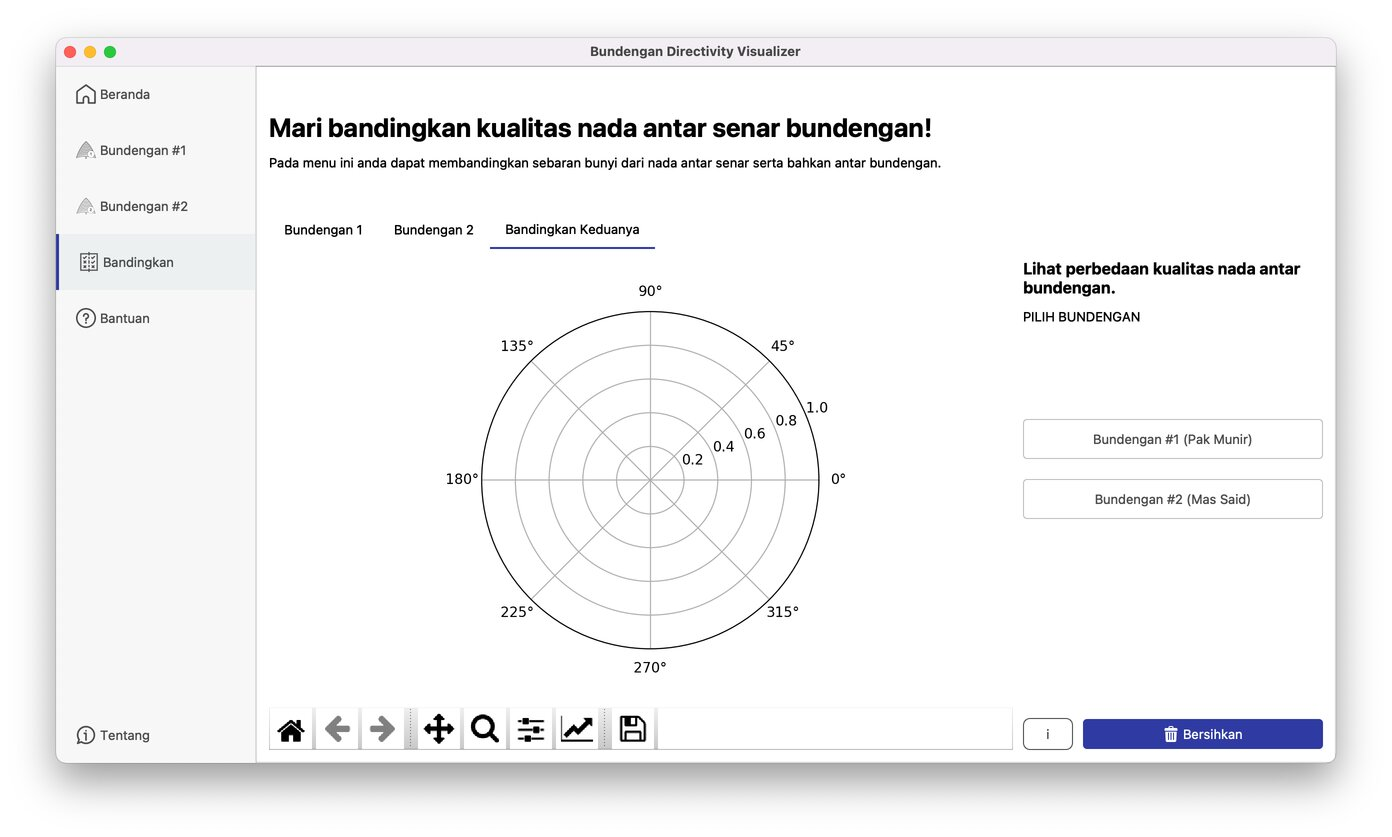
\includegraphics[width=14cm]{Gambar/laman-bandingkan.jpg}
	\caption{Tampilan laman fitur perbandingan frekuensi alami.}
	\label{fig:compare-app}
\end{figure}

Laman Bantuan berisi beberapa penjelasan terkait model visualisasi yang ditampilkan. Penjelasan dimulai dari mengenalkan \bundengan apa saja yang ada pada program dan proses pengukuran data dengan menunjukkan susunan mikrofon seperti pada Gambar \ref{fig:bundenganBatasanMasalah}. Setelah pengguna melihat posisi \bundengan relatif terhadap penempatan mikrofon, disampaikan bahwa setiap frekuensi alami (disampaikan dalam istilah "nada") ditampilkan dalam bentuk pola garis pada bidang yang sama persis dengan kondisi perekaman. Setelah itu dijelaskan apa maksud dari ditampilkannya grafik kontur, yaitu supaya pengguna dapat melihat bagaimana data keseluruhan yang terekam dan juga dapat melihat bagaimana frekuensi alami \bundengan terlihat jelas berada di antara derau yang ikut terekam. Setiap penjelasan mengenai model visualisasi dilengkapi dengan petunjuk bagaimana membaca model visualisasi tersebut. Pada Gambar \ref{fig:help-app} diperlihatkan laman bantuan yang menjelaskan bagaimana cara membaca plot diagram polar. \par 

\begin{figure}[t!]
	\centering
	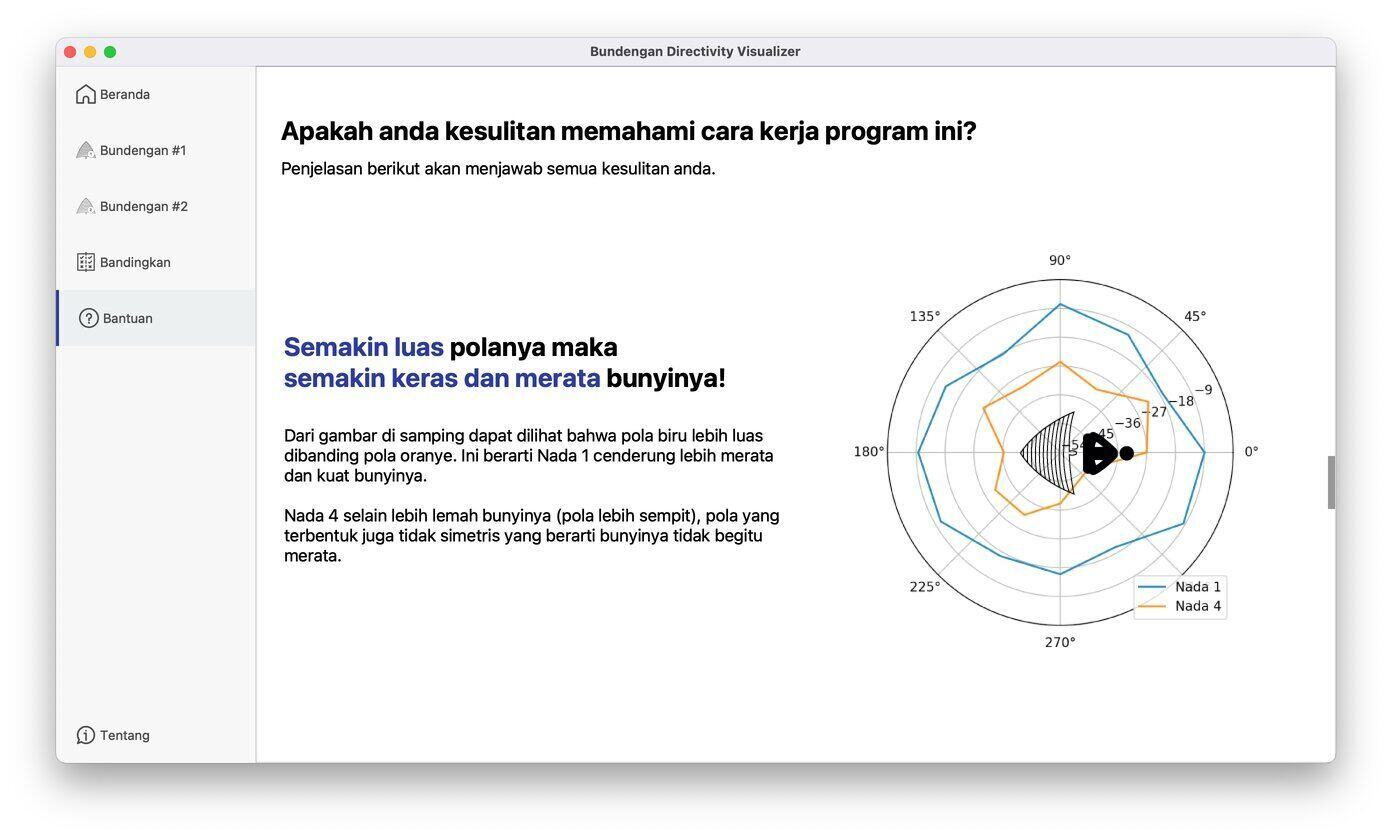
\includegraphics[width=13cm]{Gambar/laman-help.jpg}
	\caption{Tampilan laman Bantuan BundenganDVis.}
	\label{fig:help-app}
\end{figure}

Antarmuka BundenganDVis dibangun menggunakan QtDesigner, yaitu sebuah program yang membantu memudahkan pembangunan antarmuka berbasis Python menggunakan modul PyQt. Dengan QtDesigner setiap elemen grafis seperti tombol, tab, halaman, kotak centang, warna, dan teks disusun sedemikian sehingga tampak seperti yang direncanakan. Setiap elemen diberi nama khusus karena akan menjadi sebuah variabel objek ketika proses penyusunan kontrol program. \par 

Proses terakhir dari pembangunan BundenganDVis adalah menghubungkan model visualisasi dengan antarmuka yang telah dibangun. Proses ini dimulai dari mengatur fungsi untuk setiap tombol sampai dengan menampilkan model visualisasi pada area antarmuka yang telah disediakan. Seluruh proses ini dibangun menggunakan bahasa pemrograman Python. Setelah program berjalan dengan semestinya, program diekspor ke dalam format yang dapat dieksekusi oleh komputer yang tidak terpasang bahasa pemrograman Python dan pustaka-pustaka yang digunakan (.exe). Tayangan penggunaan BundenganDVis dapat dilihat dengan mengakses tautan yang terdapat pada Lampiran A. Pada halaman tersebut juga terdapat tautan untuk mengunduh BundenganDVis. \par 


\section{Pengujian Sistem oleh Calon Pengguna}
Untuk mengetahui apakah BundenganDVis bekerja dengan baik saat di kemudian hari digunakan dalam perancangan pementasan \emph{bundengan}, perlu dilakukan pengujian kinerja oleh calon pengguna. Penulis meminta lima orang responden untuk menggunakan program BundenganDVis di perangkat pribadi. Untuk pengujian sebuah sistem yang melibatkan pengalaman pengguna, lima responden adalah jumlah yang tepat untuk sistem dengan segmentasi pengguna yang sempit \cite{5user}. Hal ini untuk menghindari hasil penilaian serupa yang berulang. \par 

Idealnya pada pengujian ini responden adalah representasi pengguna, yaitu para pemusik \bundengan yang cukup familiar dengan teknologi komputer. Akan tetapi, akibat dari \bundengan yang begitu terancam punah penulis kesulitan mendapatkan responden dengan kriteria tersebut. Hanya satu responden yang sesuai dengan kriteria pengguna, yaitu narasumber yang diwawancarai ketika proses identifikasi kebutuhan pengguna. Empat responden lainnya adalah orang-orang yang cukup familiar dengan musik namun minim pengetahuan mengenai ilmu akustika. Hal ini supaya penilaian dari keempat responden tersebut mampu mewakili penilaian calon-calon musisi \bundengan baru yang juga minim pengetahuan mengenai ilmu akustika. \par 

\newpage
Setelah responden menggunakan BundenganDVis, penulis melakukan survei berbasis SUS. Proses penggunaan dan penilaian dilakukan responden tanpa ada intervensi dan bantuan dari penulis. Berikut adalah total skor SUS untuk masingmasing responden beserta interpretasinya berdasarkan rentang pada Gambar \ref{fig:SUSAdjective}:
\begin{enumerate}
	\item Responden pertama adalah mahasiswa Teknik Informatika yang hanya seorang pendengar musik. Ia memberi penilaian dengan total skor SUS sebesar 57,5. Nilai ini menunjukkan kinerja BundenganDVis bersifat "GOOD" dan masih dapat diterima.
	\item Responden kedua adalah pemusik \bundengan yang diwawancara pada saat identifikasi kebutuhan pengguna. Beliau memberi penilaian dengan total skor SUS sebesar 60. Nilai ini menunjukkan kinerja BundenganDVis bersifat "GOOD" dan masih dapat diterima.
	\item Responden ketiga adalah sarjana Teknik Kimia yang hobi bermain alat musik perkusi. Ia memberi penilaian dengan total skor SUS sebesar 92,5. Nilai ini menunjukkan kinerja BundenganDVis bersifat "BEST IMAGINABLE" dan dapat diterima.
	\item Responden keempat adalah karyawan swasta yang hobi bermain gitar. Ia memberi penilaian dengan total skor SUS sebesar 80. Nilai ini menunjukkan kinerja BundenganDVis bersifat "EXCELLENT" dan dapat diterima.
	\item Responden keempat adalah karyawan swasta yang hobi bermain \emph{keyboard}. Ia memberi penilaian dengan total skor SUS sebesar 80. Nilai ini menunjukkan kinerja BundenganDVis bersifat "EXCELLENT" dan dapat diterima.
\end{enumerate}
Nilai yang diberikan setiap responden pada tiap pertanyaan dapat dilihat melalui tautan pada Lampiran A. Dari seluruh nilai SUS yang diberikan oleh responden, rata-rata total skor yang didapat oleh BundenganDVis adalah 74 dengan nilai simpangan baku 14,9. Nilai ini menunjukkan bahwa BundenganDVis masih dapat diterima oleh pengguna dengan latar belakang ilmu akustika yang minim. Meskipun demikian, nilai yang diberikan oleh responden pertama dan kedua menunjukkan bahwa pengguna dengan latar belakang ilmu sains yang sangat minim tetap perlu bimbingan ketika menggunakan BundenganDVis. \par 

